\section{Обзор численных методов \label{methods}}
В этой главе мы рассматриваем методы численного решения нелинейных уравнений, которые применялись в рамках данной работы. Методы использовались для решения уравнения теплопроводности \eqref{eq:heat_equation_intro} и системы функционала плотности \eqref{eq:dhd_system_intro}. Выбор именно этих методов обусловлен гладкостью всех функций, составляющих исследуемые задачи. Мы не рассматриваем разрывные решения и ударные волны.
\par 
Для простоты применение методов объясняется на примере уравнения теплопроводности, однако это не ограничивает сферу их применения.
\subsection{Аппроксимация производной по пространству \label{methods:space_derivative}}
Область $D$ разбивается по каждому направлению с равномерным шагом $h_i$, образуя сетку $\{x_m\}; \quad m = \overline{0 \dots M-1}$. В многомерном случае сетка получается декартовым произведением одномерных сеток. Мы применяем метод 2 порядка аппроксимации по пространству.  Для этого используется формула центральной разности, которая вычисляет значение производной в точке посередине между соседними точками сетки. По каждой оси вводятся вспомогательные сетки $\{ x_{m+0.5}\}$,  $\{ y_{m+0.5}\}$ и  $\{ z_{m+0.5}\}$, где $m = \overline{0 \dots M-2}$. Узлы находятся между узлами обычной сетки по данной оси:
\begin{equation}
x_{m + 0.5} = \frac{x_m + x_{m+1}}{2};
\quad
y_{m + 0.5} = \frac{y_m + y_{m+1}}{2};
\quad
z_{m + 0.5} = \frac{z_m + z_{m+1}}{2}
\end{equation}

\par
Продемонстрируем пользу дополнительной сетки на примере одномерного уравнения теплопроводности \eqref{eq:heat_equation_intro}. Мы используем для внутренней производной формулу центральной разности со 2 порядком аппроксимации, производная находится в узлах сетки $\{ x_{m+0.5}\}$:
\begin{equation}
\left.\frac{\partial u}{\partial x_i} \right\vert_{m+0.5}= \frac{u_{m+1} - u_m}{h} + O(h^2)
\end{equation}
Оператор дифференцирования по пространству в одномерном уравнении теплопроводности имеет такой вид:
\begin{equation}
\frac{\partial}{\partial x} \left( \alpha(u) \frac{\partial u}{\partial x}\right)
\end{equation}
Для вычисления $\alpha(u)$ на $\{ x_{m+0.5}\}$ используем линейную интерполяцию, поскольку функции $\alpha$ и $u$ непрерывны:
\begin{equation}
\alpha_{m+0.5} = \alpha(\frac{u_{m+1} + u_{m}} {2});
\quad 
\alpha_{m-0.5} = \alpha(\frac{u_{m} + u_{m - 1}} {2})
\end{equation}
Внешняя производная переводит значения снова на сетку $\{ x_m \}$ по формуле центральной разности. Таким образом, дискретизация оператора имеет вид:
\begin{equation}
\frac{\partial }{\partial x} \left( \alpha (u) \frac{\partial u}{\partial x} \right)  = \frac{1}{h_x} \left( \alpha_{m+0.5} \frac{u_{m+1} - u_m}{h_x} - \alpha_{m-0.5} \frac{u_{m} - u_{m-1}}{h_x} \right) + O(h_x^2)
\end{equation}
Благодаря дополнительной сетке мы достигаем 2 порядка аппроксимации производных по пространству.
\subsection{Интегрирование по времени \label{methods:time_integration}}
Перейдем к аппроксимации производной по времени. В рассматриваемых в данной работе задачах используется только первая производная по времени. Поэтому после дискретизации по пространству все эти задачи можно представить в виде:
\begin{equation} \label{eq:time_problem_general}
\frac{\partial \vec u}{\partial t} + F(\vec u) = 0
\end{equation}
где $\vec u$ - значения всех неизвестных в узлах сетки, а $F(\vec u)$ - некоторый нелинейный оператор, включающий в себя производные по пространству. 
\par
Введем сетку по времени $\{t_n\}$ разбиением отрезка $[0, T]$ на неравномерные шаги $\tau_n$. Будем использовать обозначение $\vec {u^n}$ для численного решения на неизвестном слое по времени, $\vec{u^{n - k}}$, $k \in \mathbb{N}$ - для известных. Когда номер шага $\tau_n$ понятен из контекста, будем использовать символ $\tau$ без индекса.
\par
Методы аппроксимации производной по времени делятся на 2 типа: \textit{явные} и \textit{неявные}. \textit{Явные методы} аппроксимируют производную по времени на слое $n - 1$:  $\left. \frac{\partial \vec u}{\partial t} \right \vert_{n-1} \approx F(\vec {u^{n-1}})$. Применение явного метода дает вид формулы, по которой можно вычислить $\vec{u^n}$. \textit{Неявные методы} аппроксимируют производную на неизвестном слое $n$ или между известным и неизвестным слоем: $\left. \frac{\partial \vec u}{\partial t} \right\vert_{n} \approx F(\vec {u^{n}})$. Функция в правой части зависит от значений на неизвестном слое. Необходимо решать систему уравнений относительно $\vec{u^n}$.
\subsubsection{Явный метод Эйлера}
\begin{equation}
\left. \frac{\partial \vec u}{\partial t} \right \vert_{n - 1} = \frac{\vec {u^n} - \vec {u^{n-1}}}{\tau} + O(\tau)
\end{equation}
Как известно, для явных методов шаг по времени  $\tau$ ограничивается условием устойчивости. Например, для линейного уравнения теплопроводности:
\begin{equation}
\alpha \cdot \tau \leq \frac{1}{2} \left( \sum_{a=1}^d \frac{1}{h_a^2}\right)^{-1}
\end{equation}
где $d$ - размерность пространства. Вывод условия устойчивости приведен в \cite{Samarskii}.
\subsubsection{Неявный метод Эйлера}
\begin{equation}
\left. \frac{\partial \vec u}{\partial t} \right \vert_{n} = \frac{\vec {u^n} - \vec {u^{n-1}}}{\tau} + O(\tau)
\end{equation}
\subsubsection{Трехточечная односторонняя разность второго порядка точности \label{methods:back-diff}}
Неявный метод Эйлера позволяет устойчиво делать большие шаги по времени, но его первый порядок по времени во многих случаях дает слишком малую точность. Поэтому мы также рассматриваем методы второго порядка по времени.
\begin{equation} 
\left. \frac{\partial \vec u}{\partial t} \right \vert_{n} = \frac{3 \vec {u^{n}} - 4 \vec {u^{n - 1}} + \vec {u^{n - 2}}} {2 \tau} + O(\tau^2)
\end{equation}
Данный метод является неявным. Он использует 2 предыдущих временных слоя, которые нужно хранить в памяти. Первый шаг делается \textit{методом Эйлера}. В \cite{Samarski-intro} доказывается абсолютная устойчивость этого метода.
\subsubsection{Метод Кранка-Николсона}
Можно получить 2 порядок аппроксимации по времени, не храня в памяти 3 временных слоя. Для этого производная по времени вычисляется по формуле центральной разности в точке: $t_{n-0.5} = \frac{t_{n} + t_{n-1}}{2}$. Формула центральной разности дает 2 порядок аппроксимации: 
\begin{equation}
\left. \frac{\partial \vec {u}}{\partial t} \right \vert_{n-0.5} = \frac{\vec {u^n} - \vec {u^{n-1}}}{\tau} + O(\tau ^ 2)
\end{equation}
Чтобы метод работал правильно, нужно взять правую часть уравнения \eqref{eq:time_problem_general} в момент времени $n-0.5$. 
Для источника $\vartheta$ это легко, поскольку он определен аналитически. Пространственную производную нужно будет интерполировать, так как мы получаем ее численно из значений на каждом временном слое:
\begin{equation}
\left. \frac{\partial \vec u}{\partial x} \right \vert_{n-0.5} = \frac{1}{2}\left( \left. \frac{\partial \vec u}{\partial x} \right \vert_{n} + \left. \frac{\partial \vec u}{\partial x} \right \vert_{n - 1} \right)
\end{equation}
Поэтому данный метод относится к \textit{неявным}. Он абсолютно устойчив, однако обладает ограничением асимптотической устойчивости. Для уравнения теплопроводности оно имеет такой вид:
\begin{equation}
\tau < \tau_0,
\quad
\tau_0 \approx \frac {h}{\pi}
\end{equation}
Данное условие получено в \cite{Samarski-intro}. Нарушение условия асимптотической устойчивости может приводить к нежелательным осцилляции в решении. Метод \ref{methods:back-diff} не накладывает такое условие.

\subsection{Подходы к решению многомерных неявных по времени задач}
Использование неявного метода интегрирования по времени приводит к нелинейной системе уравнений. Метод ее решения, который мы используем в данной работе, будет описан в разделе \ref{methods:newton}. Важно, что он представляет из себя многократное решение систем линейных уравнений на основе матрицы Якоби. 
\par 
Некоторые матрицы обладают определенной  \textit{тридиагональной} структурой. Как будет показано позже в разделе \ref{methods:tridiagonal}, систему с такой матрицей можно решить очень быстро. Вид тридиагональной матрицы приводится в \eqref{mat:tridiagonal}.
Тридиагональной структурой обладает, например, матрица Якоби одномерного уравнения теплопроводности \eqref{eq:heat_equation_intro}. Двумерное и трехмерное уравнения теплопроводности такой структурой не обладают, как и одномерная векторная система функционала плотности. 
\par
Во многих реальных задачах матрица не обладает тридиагональной структурой. Можно попытаться разбить каждый шаг по времени на несколько задач, каждая из которых будет сводиться к решению тридиагональной системы, либо использовать методы, не требующие тридиагональной структуры. Такие методы всегда будут требовать значительно больше операций. Таким образом, мы выделили 2 подхода к решению: 
\begin{enumerate}
\item Разбить на подзадачи
\item Использовать метод, не требующий тридиагональной структуры
\end{enumerate}
Покажем на примере, как разделять шаг по времени на подзадачи.
\subsubsection*{Метод переменных направлений \label{methods:alternate_directions}}
Решаем двумерное уравнение теплоповодности \eqref{eq:heat_equation_intro}. Шаг по времени разбивается на 2 части. Первая часть неявна по направлению $x$, а вторая - по $y$. Сначала методом прогонки вычисляются промежуточные значения $\tilde u$ в момент времени $t_{n - 0.5}$. Затем методом прогонки вычисляются значения $u^n$, используя известные $\tilde u$:
\begin{equation}
\begin{cases}
\tilde u_{mk} = f_1(\tilde u_{m, k \pm i}, u^{n - 1}_{m \pm i, k} ) 
\\ \\
u^{n}_{mk} = f_2(\tilde u_{m, k \pm i}, u^{n}_{m \pm i, k} )
\end{cases}
\quad i = 0, \pm 1
\end{equation}
Данный метод абсолютно устойчив, однако его трехмерный аналог неустойчив. Исследование устойчивости проводится в \cite{Sikovskii}.

\subsection*{}
Главный недостаток подхода, разбивающего шаг по времени на подзадачи - трудность его обобщения. Для каждой конкретной задачи нужно разрабатывать методы разбиения системы. После этого нужно исследовать разработанный метод на устойчивость. Если решается система более сложного вида, чем уравнение теплопроводности, разработка такого подхода сложна. Однако, если удастся получить и обосновать такой подход, вычислительная нагрузка при решении задачи сократится в разы. Мы не будем подробно останавливаться на разработке таких методов. Сосредоточимся на более общем подходе - будем решать разреженную систему, не привязываясь к ее конкретному виду.

\subsection{Решение нелинейных систем уравнений \label{methods:newton}}
Использование неявного метода интегрирования по времени приводит к нелинейной системе уравнений из $M$ уравнений с $M$ неизвестными вида:
\begin{equation}\label{eq:newtons_method_system}
\mathbf{F}(\mathbf{x}) = \mathbf{0}
\end{equation}
Для решения таких систем мы решили остановиться на \textit{методе Ньютона}, как на наиболее робастном методе для нашего типа задач. 
\subsubsection*{Метод Ньютона} Ищем точное решение $\mathbf{\tilde x}$ уравнения \eqref{eq:newtons_method_system}. Возьмем начальное приближение решения $\mathbf{x_0}$. Разложим в ряд Тейлора в окрестности $\mathbf{\tilde x}$ функцию $\mathbf{F}(\mathbf{x_0)}$:
\begin{equation}
\mathbf{F}(\mathbf{\tilde x}) \approx \mathbf{F}({\mathbf{x_0}}) + \mathbf{J}(\mathbf{x_0}) \cdot (\mathbf{\tilde x} - \mathbf{x_0})
\end{equation}
Здесь $\mathbf{J}$ - матрица Якоби (матрица частных производных по $\mathbf{x}$ функции $\mathbf{F}$). Заменим $\Delta \mathbf{x} = \mathbf{\tilde x} - \mathbf{x_0}$:
\begin{equation}
\mathbf{J}(\mathbf{x_0}) \cdot \Delta \mathbf{x} = - \mathbf{F}(\mathbf{x_0})
\end{equation}
Получаем систему уравнений, позволяющую приблизиться на $\Delta \mathbf{x}$ к искомому решению. Одной итерации алгоритма недостаточно, так как окрестность может быть не малой. Из-за этого в разложении в ряд Тейлора будет большая ошибка. Сделаем несколько таких итераций. Запишем итерационную формулу для последовательности $\mathbf{x^n}$, приближающейся к $\mathbf{\tilde x}$:
\begin{equation} \label{eq:newton_method}
\mathbf{J}(\mathbf{x^n}) \cdot \Delta \mathbf{x^n} = - \mathbf{F}(\mathbf{x^n})
\end{equation}
Критерием остановки является малость нормы невязки $\mathbf{F}(\mathbf{x^n}) = \mathbf{r^n};
\quad ||\mathbf{r^n}||< C$.
\par
Систему можно переписать в виде $\Delta \mathbf{x^n} = - \mathbf{J^{-1}}(\mathbf{x^n}) \cdot \mathbf{F}$. Тогда задача сводится к поиску обратной матрицы $\mathbf{J^{-1}}$. На практике легче решать именно систему, пользуясь ее разреженной структурой, а не искать обратную матрицу.
\subsubsection*{Применение метода Ньютона}
На каждой итерации метода Ньютона необходимо:
\begin{enumerate}
\item Вычислить матрицу Якоби для нелинейной системы
\item Решить систему линейных уравнений
\end{enumerate}
Оптимизации 1-го действия будут рассмотрены в главе \ref{implementation:operator_preconditioning}. Основная вычислительная нагрузка в методе Ньютона заключается в решении линейной системы уравнений, так как размерность матрицы $M \times M$ может быть очень большой. Выбор эффективного метода решения линейной системы - залог эффективности решения нелинейной задачи.

\subsection{Решение линейных систем алгебраических уравнений \label{methods:linear_solvers}}
Для метода Ньютона нам необходимо решать системы линейных алгебраических уравнений (СЛАУ)
общего вида:
\begin{equation} \label{eq:linear_system}
\mathbf{Ax} = \mathbf{b}
\end{equation}
Разделяют \textit{прямой} и  \textit{итерационный} подход к решению. \textit{Прямые} методы позволяют получить точное решение с погрешностью только от округления чисел с плавающей запятой. Количество операций в таких методов быстро растет с увеличением размера системы. Поэтому их применение для больших систем может быть неоправданно долгим. \textit{Итерационные} методы образуют последовательность приближенных решений, которая сходится к точному. Итерации можно остановить, если достигнута требуемая точность решения. Рассмотрим сначала \textit{прямые} методы, использованные в данной работе, потом \textit{итерационные}. В конце рассмотрим подробно методы \textit{подпространства Крылова} - особый класс методов.
\paragraph{Подпространством Крылова} называется линейное пространство
\begin{equation} \label{eq:krylov_subspace}
K_m(v, \mathbf{A}) = span\left\{ v, \mathbf{A}v, \mathbf{A}^2v, \dots, \mathbf{A}^{m-1}v \right\}
\end{equation}
Принцип действия рассматриваемых методов был впервые предложен в работе \cite{Krylov}.
Методы строят решение в \textit{подпространстве Крылова}. Одно из преимуществ таких методов - они позволяют не хранить численное представление матрицы $\mathbf{A}$. Достаточно знать, как она действует на произвольный вектор. Этот подход называется \textit{безматричным}. Методы подпространства Крылова могут быть как итерационными, так и прямыми.

\subsubsection{Алгоритм прогонки \label{methods:tridiagonal}}
Данный метод прямой. Он применяется, если матрица $\mathbf{A}$ имеет тридиагональный вид:
\begin{equation} \label{mat:tridiagonal}
\left[
\begin{array}{ccccccccc}
\times & \times & 0 & \ddots \\
\times & \times  & \times & 0 & \ddots \\
0 & \times & \times & \times & 0 & \ddots \\
\ddots & 0 & \times & \times & \times & 0 & \ddots \\
& \ddots & 0 & \times & \times & \times & 0 & \ddots \\
&& \ddots & 0 & \times & \times & \times & 0 \\
&&& \ddots & 0 & \times & \times & \times \\
&&&& \ddots & 0 & \times & \times\\
\end{array}
\right]
\end{equation}
где $\times$ - ненулевой элемент.
Такой вид имеет, например, матрица Якоби в одномерной задаче теплопроводности \eqref{eq:heat_equation_intro}.
В системе с тридиагональной матрицей неизвестные компоненты вектора $x$ связаны соотношениями:
\begin{equation}
A_i x_{i-1} + B_i x_i + C_i x_{i+1} = F_i
\end{equation}
По индукции можно показать, что справедливо:
\begin{equation}
x_i = \alpha_{i+1} x_{i+1} + \beta_{i+1}
\end{equation}
Можно выразить коэффициенты $\alpha_i$ и $\beta_i$ через $A_i, B_i, C_i$:
\begin{equation}
\begin{cases}
\alpha_2 = \frac{-C_1}{B_1} \\
\beta_2 = \frac{F_1}{B_1}
\end{cases}
\end{equation}
\begin{equation}
\begin{cases}
\alpha_{i+1} = \frac{-C_i}{A_i \alpha_i + B_I} \\
\beta_{i+1} = \frac{F_1 - A_i \beta_i}{A_i \alpha_i + B_i}
\end{cases}
\end{equation}
Нахождение этих коэффициентов равносильно преобразованию матрицы $\mathbf{A}$ к треугольному двудиагональному виду. Зная коэффициенты $\alpha_i$ и $\beta_i$ можно найти $x_i$. Метод прогонки позволяет найти решение за $O(M)$, где $M$ - количество элементов $x_i$. Метод рассматривается подробнее в \cite{Petrov}.

\subsubsection{Разложение Холецкого \label{methods:cholesky}}
Данный метод прямой. Если матрица симметрична и положительно определена, ее можно представить разложением Холецкого: $\mathbf{A} = \mathbf{LL}^T$ , где $\mathbf{L}$ - нижняя треугольная матрица. Систему линейных уравнений с треугольной матрицей можно эффективно решить. 
Найдя матрицу $L$, решение системы \eqref{eq:linear_system} сводится к решению 2-х систем с треугольными матрицами:
\begin{equation}
    \mathbf{L} \cdot \mathbf{y} = \mathbf{a};
    \quad
    \mathbf{L}^T \cdot \mathbf{x} = \mathbf{y}
\end{equation}
Алгоритм разложения приведен в \cite{Petrov}.

\subsubsection{Разложение LU \label{methods:lu}}
Данный метод прямой. Исходную матрицу можно разложить нижнюю $\mathbf{L}$ и верхнюю $\mathbf{U}$ треугольные матрицы. Метод применим к произвольной матрице, если она обратима, и все главные миноры невырождены. Получив матрицы $\mathbf{L}$ и $\mathbf{U}$, можно получить $\mathbf{x}$, решив 2 треугольные системы:
\begin{equation}
    \mathbf{L} \cdot \mathbf{y} = \mathbf{a};
    \quad
    \mathbf{U} \cdot \mathbf{x} = \mathbf{y}
\end{equation}
Алгоритм разложения приведен в \cite{Petrov}.

\subsubsection{Метод неполного разложения \label{methods:ilu}}
Применим \textit{разложение LU} (раздел \ref{methods:lu}) для разреженной матрицы. Результаты $\mathbf{L}$ и $\mathbf{U}$ не будут повторять шаблон разреженности исходной матрицы. Для ускорения расчета хотелось бы получить разреженные факторизации. Можно найти такое примерное разложение $\mathbf{A} \approx \mathbf{LU}$, где $\mathbf{L}$  и $\mathbf{U}$ - нижняя и верхняя тридиагональные матрицы, равные нулю там, где ${A}_{ij} = 0$. Для этого применяется такой же алгоритм, как для полного разложения. Однако вычисляются только те ячейки, где ${A}_{ij} \neq 0$, а остальные считаются равными $0$.  Это значительно ускоряет поиск факторизации для разреженной матрицы. Такой метод называют \textbf{ILU}.
\par
Можно изменить шаблон разреженности, например, сделать матрицы более полными. Это замедлит поиск факторизации, но сделает решение точнее. Золотая середина между скоростью и эффективностью подбирается экспериментально. Аналогичным образом можно получить разреженное разложение для \textit{метода Холецкого} (раздел \ref{methods:cholesky}). Более подробное описание дано в \cite{Golub}.

\subsubsection{Метод Якоби}
Данный метод итерационный. Пусть $\mathbf{D} = diag(\mathbf{A})$, $\mathbf{L}$ и $\mathbf{U}$ - нижняя и верхняя треугольные матрицы, $\mathbf{A} = \mathbf{D} + \mathbf{L} + \mathbf{U}$. Если $A_{ii} \neq 0$, систему \eqref{eq:linear_system} можно представить в виде $\mathbf{x} = \mathbf{Bx} + \mathbf{g}$, где $\mathbf{B} = \mathbf{D}^{-1} (\mathbf{D} - \mathbf{A})$. Тогда алгоритм поиска решения будет иметь вид:
\begin{equation}
x_i^{(k+1)} = \frac{1}{a_{ii}} \left( b_i - \sum_{j \neq i} a_{ij} x_j^{(k)} \right)
\end{equation}
Метод рассматривается подробнее в \cite{Petrov}. Одним из главных преимуществ метода Якоби является его сглаживающее свойство, что позволяет его эффективно использовать в многосеточном методе \ref{methods:multigrid}.

\subsubsection{Метод Гаусса-Зейделя \label{methods:gauss_seidel}}
Данный метод итерационный. Он является модификацией \textit{метода Якоби}. Метод использует только что полученные значения, $x_i^{(k+1)}$ для нахождения $x_{i+1}^{(k+1)}$. Решаемая система выглядит таким образом:
\begin{equation}
(\mathbf{L} + \mathbf{D}) \mathbf{x}^{(k+1)} = -\mathbf{Ux}^{(k)} + \mathbf{b}
\end{equation}
Метод рассматривается подробнее в \cite{Petrov}. Данный метод также обладает сглаживающим свойством.

\subsubsection{Многосеточной метод (Multigrid) \label{methods:multigrid}}
Данный метод итерационный. Суть алгоритма состоит в решении задачи на разных сетках. Сетки последовательно становятся грубее, уменьшая размерность системы. Для интерполяции  результатов на более грубые сетки и назад заранее выбираются операторы интерполяции. На каждой сетке применяется выбранный итерационный метод решения системы линейных уравнений, например, \textit{метод Гаусса-Зейделя} (раздел \ref{methods:gauss_seidel}). Выбранный метод применяется не полностью, делаются только первые несколько итераций. Этот процесс называется \textit{сглаживанием}.
\paragraph{Алгоритм задается рекуррентно:}
\begin{itemize}
\item Сделать $k$ итераций сглаживания
\item Интерполировать $\mathbf{A}$ и $\mathbf{b}$ на более грубую сетку
\item Если мы не достигли самой грубой сетки: 
\begin{itemize}
\item Получить невязку $\mathbf{r}$ на более грубой сетке с помощью \textit{Многосеточного метода}
\item Интерполировать $\mathbf{r}$ на менее грубую сетку и вычесть ее 
\end{itemize}
\item Сделать $k$ итераций сглаживания
\end{itemize}
Число $k$ и количество грубых сеток выбираются заранее. 
\par
Преимущество данного метода заключается в том, что он действует на разные масштабы невязки, подавляя ее разные гармоники. Обычные итерационные методы плохо подавляют ''низкочастотную'' невязку. Количество операций линейно возрастает с увеличением размера задачи. 
\par
Возможен разный вид циклов \textit{Многосеточного метода}. Алгоритм, описанный выше, называется \textit{V-цикл}. Есть и другие известные вариации алгоритма - \textit{F-цикл} и \textit{W-цикл}. Структуры алгоритмов приведены на рис. \ref{fig:multigrid}. Разные циклы имеют разные свойства сходимости и применимы к разным задачам. Подробнее этот вопрос рассматривается в \cite{briggs2000multigrid}.
\begin{figure}[H]
\centering
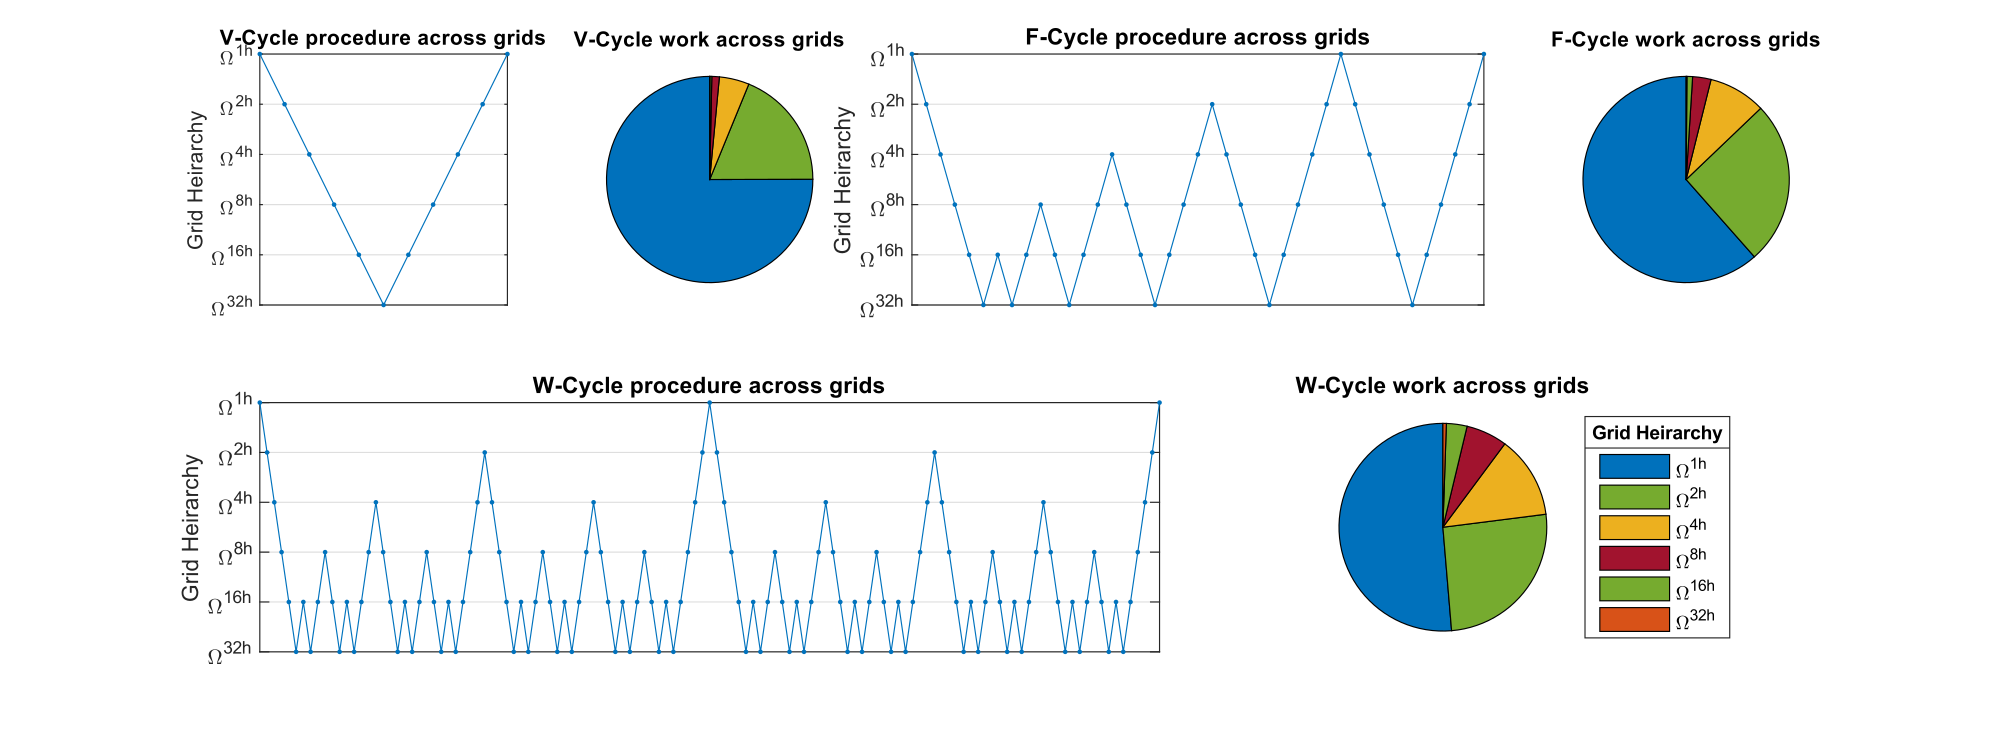
\includegraphics[width=\textwidth]{common_images/MultigridWork.png}
\caption{Различные циклы Многосеточного метода. \begin{small}(Источник: \url{https://commons.wikimedia.org/wiki/File:MultigridWork.svg})\end{small}}
\label{fig:multigrid}
\end{figure}

\subsubsection{Метод сопряженных градиентов \label{methods:conjugate_gradients}}
\paragraph{Прямой подход}
Данный метод относится к методам подпространства Крылова.
Пусть $\mathbf{A}$ - симметричная, положительно-определенная матрица, а $\mathbf{x_*}$ - решение исходной системы. Будем приближаться к решению \textit{сопряженными} шагами. \textit{Сопряженными} относительно матрицы $\mathbf{A}$ называются такие векторы $\mathbf{u}$ и $\mathbf{v}$, что  $\mathbf{u^T A v} = 0$. Решение можно представить через набор сопряженных векторов $P = \{ \mathbf{p_1}, ..., \mathbf{p_n} \}$, они образуют базис подпространстве Крылова \eqref{eq:krylov_subspace}. Тогда искомое решение имеет вид:
\begin{equation}
\mathbf{x_*} = \sum^n_{i=1} \alpha_i \mathbf{p_i}
\end{equation}
Домножим его на $\mathbf{A}$:
\begin{equation}
\mathbf{A x_*} = \sum^n_{i=1} \alpha_i \mathbf{A p_i}
\end{equation}
Домножим на $\mathbf{p_k^T}$, пользуясь сопряженностью $\mathbf{p}$:
\begin{equation}
\mathbf{p}^T_k \mathbf{A} \mathbf{x_*} = \alpha_k \mathbf{p_k}^T \mathbf{A} \mathbf{p_k}
\end{equation}
Воспользуемся \eqref{eq:linear_system}, выразим $\alpha_k$:
\begin{equation}
\alpha_k = \frac{\mathbf{p}^T_k \mathbf{b}}{\mathbf{p_k}^T \mathbf{A} \mathbf{p_k}}
\end{equation}
Для точного решения нужно найти $n$ базисных векторов $\mathbf{p}_k$ и коэффициентов $\alpha_k$.

\paragraph{Итерационный подход}
Если удачно выбрать несколько первых базисных векторов $\mathbf{p}_k$, можно не делать все $n$ шагов
для получения решения с нужной точностью. Итерационный подход рассматривает решение системы как задачу
минимизации функции
\begin{equation}
f(\mathbf{x}) = \frac{1}{2} \mathbf{x}^T \mathbf{A} \mathbf{x} - \mathbf{x}^T \mathbf{b}
\end{equation}
где минимум $\mathbf{x_*}$ cуществует, поскольку вторая производная $\nabla ^2 f(\mathbf{x}) = \mathbf{A}$ симметрична и положительно определена. Градиентом функции является невязка исходной задачи:
\begin{equation}
\nabla f(\mathbf{x}) = \mathbf{r} = \mathbf{Ax} - \mathbf{b}
\end{equation}
Возьмем начальное приближение решения $\mathbf{x_0}$. Так как мы ищем минимум функции, можно взять первым базисным вектором отрицательный градиент в точке $\mathbf{x_0}$:
\begin{equation}
\mathbf{p}_0 = \mathbf{b} - \mathbf{Ax}_0
\end{equation}
Cледующие шаги выбираются в направлении, сопряженном ко всем предыдущим базисным векторам:
\begin{equation}
\mathbf{p}_k = \mathbf{r}_k + \sum_{i < k} \frac {\mathbf{p}^T_i \mathbf{A r}_k}
{\mathbf{p}^T_i \mathbf{A p}_i} \mathbf{p}_i
\end{equation}
где $\mathbf{r}_k = \mathbf{b} - \mathbf{Ax}_k$ - текущая невязка. Так находится приближенное решение
$\mathbf{x}_{k+1} = \mathbf{x}_k + \alpha_k \mathbf{p}_k$.
\\ \\
Коэффициент $\alpha_k$ находится из минимизации $f(\mathbf{x}_{k+1})$ по параметру $\alpha_k$. Пользуемся $f(\mathbf{x}_{k+1}) = f(\mathbf{x}_k + \alpha_k \mathbf{p}_k) = g(\alpha_k)$, требуем $g'(\alpha) = 0$. Отсюда:
\begin{equation}
\alpha_k = \frac {\mathbf{p}^T_k (\mathbf{b} - \mathbf{A x}_k)} {\mathbf{p}^T_k \mathbf{A} \mathbf{p}_k}
\end{equation}
\par
Метод сопряженных градиентов может быть преобразован в форму, не требующую хранения в памяти всех базисных векторов $\mathbf{p}_k$. Сходимость метода оценивается в \cite{Golub}.
\par
Главный недостаток метода - матрица должна быть симметрична и положительно определена. В уравнении теплопроводности \eqref{eq:heat_equation_intro} эти требования выполняются. В системе \textit{функционала плотности} \eqref{eq:dhd_system_intro} они могут не выполняться. Поэтому необходимо рассмотреть другие методы, которые не накладывают такие ограничения.

\subsubsection{Метод обобщенных минимальных невязок (GMRES) \label{methods:gmres}}
Данный метод относится к методам подпространства Крылова.
Решение приближается через вектор в \textit{подпространстве Крылова} с минимальной невязкой. Подпространство строится по вектору невязки: $K_n = K_n(A, r_0)$, где $r_0 = b - Ax_0$, $x_0$ - начальное приближение. Точное решение приближается вектором $x_n \in K_n$, с которым невязка $r_n$ минимальна.
\par
Векторы $r_0, A r_0, \dots A^{n - 1} r_0 \in K_n$  могут быть практически линейно зависимыми. Удобнее построить ортонормированный базис $q_1,\dots q_n \in K_n$  с помощью \textit{итераций Арнольди} (процесс описан в \cite{saad2003iterative}). После этого решается задача минимизации нормы невязки и строится решение исходной системы. Базисные векторы $q_1, \dots q_n$  формируют матрицу $Q_n$, по которой раскладывается решение: $x_n = Q_n y_n$. В процессе \textit{итераций Арнольди} формируется верхняя матрица Хессенберга $\tilde H_n$ размерности $(n + 1) \times n$:

\begin{equation}
A Q_n = Q_{n+1} \tilde H_n
\end{equation}
Получим выражение нормы невязки для минимизации:
\begin{equation}
||r_n|| = ||A x_n - b|| = ||\tilde H_n y_n - Q^T_{n+1} b|| = ||\tilde H_n y_n - \beta e_1||
\end{equation}
Здесь мы воспользовались тем, что $Q_n$ образуется из ортонормированного базиса векторов. $e_1$ - первый базисный вектор в начальном базисе в $\mathbb{R}^{n+1}$. $\beta = ||b - A x_0||$. Таким образом, $x_n$ можно найти, минимизируя норму невязки:
\begin{equation}
r_n = \tilde H_n y_n - \beta e_1
\end{equation}
Данная задача сводится к задаче наименьших квадратов. Приведем алгоритм n-ой итерации метода GMRES:
\begin{enumerate}
\item Вычисление нового базисного вектора \textit{методом Арнольди}
\item Нахождение $y_n$, который минимизирует невязку $||r_n||$
\item Вычисление $x_n = Q_n y_n$
\item Повторение, если невязка недостаточно мала
\end{enumerate}

Метод GMRES может быть использован с произвольной обратимой матрицей. С увеличением размерности подпространства $K_n$ увеличивается объем используемой памяти. Поэтому раз в определенное количество итераций необходимо делать рестарт с новым приближенным решением.
\par
Подробное описание метода GMRES приводится в \cite{saad2003iterative}.

\subsubsection{Метод бисопряженных градиентов}
Метод сопряженных градиентов решает только системы с симметричной матрицей. Можно модифицировать его, чтобы снять это ограничение.
Данный метод ищет невязку в подпространстве Крылова \eqref{eq:krylov_subspace} $K(v, A)$, где вектор $v$ обычно берется нормированной невязкой начального приближения. Отличие от метода сопряженных градиентов заключается в том, что вектора проекций решения строятся ортогонально подпространству Крылова $K(w, A^T)$, где $w = b^* - A^T x_0^*$. Вектор $v$ должен быть ортогонален вектору $w$. Алгоритм метода приводится в \cite{saad2003iterative}.  

\subsubsection{Стабилизированный метод бисопряженных градиентов (BiCGStab) \label{methods:bicgstab}}
Данный метод разработан на основе \textit{метода бисопряженных градиентов} и \textit{метода GMRES}, чтобы улучшить стабильность сходимости. На каждом шагу бисопряженных градиентов решается система методом GMRES с рестартом на каждой итерации.
Подробнее данный метод описывается в \cite{saad2003iterative}.

\subsubsection{Предобуславливатели \label{methods:preconditioning}}
Оценки сходимости итерационных методов проведены в \cite{briggs2000multigrid}. Они показывают, что итерационные методы работают эффективно с хорошо обусловленной матрицей. Перед решением системы можно совершить линейное преобразование и решать \textit{предобусловленную} систему. 
\paragraph{Предобуславливателем} матрицы $\mathbf{A}$ называется такая матрица $\mathbf{M}$, что $\mathbf{M} \cdot \mathbf{A} \approx \mathbf{I}$, где $\mathbf{I}$ - единичная матрица. У $\mathbf{I}$ наилучшее число обусловленности: $\mu(\mathbf{I}) = 1$. Иначе говоря, $\mathbf{M} \approx \mathbf{A^{-1}}$. \textit{Алгоритмы подпространства Крылова} не используют саму матрицу, однако каждый из них можно модифицировать, чтобы решалась предобусловленная система $\mathbf{M} \cdot \mathbf{A} \cdot x = \mathbf{M} \cdot \mathbf{b}$ или $\mathbf{A} \cdot \mathbf{M} \cdot x = \mathbf{b} \cdot \mathbf{M} $.
\par
Для произвольного численного метода в качестве предобуславливателя можно эффективно использовать полную или неполную факторизацию Холецкого или LU (раздел \ref{methods:ilu}), поскольку они позволяют получить приближение обратной матрицы в явном виде.
В качестве предобуславливателя \textit{метода подпространства Крылова} можно использовать любой численный метод решения линейной системы. Достаточно сделать несколько итераций такого метода, чтобы примерное решение системы: $\mathbf{x} \approx \mathbf{A}^{-1} \mathbf{b}$. Подробнее использование предобуславливателей описано в \cite{Golub} и \cite{saad2003iterative}.
